\section{Logische Operationen}
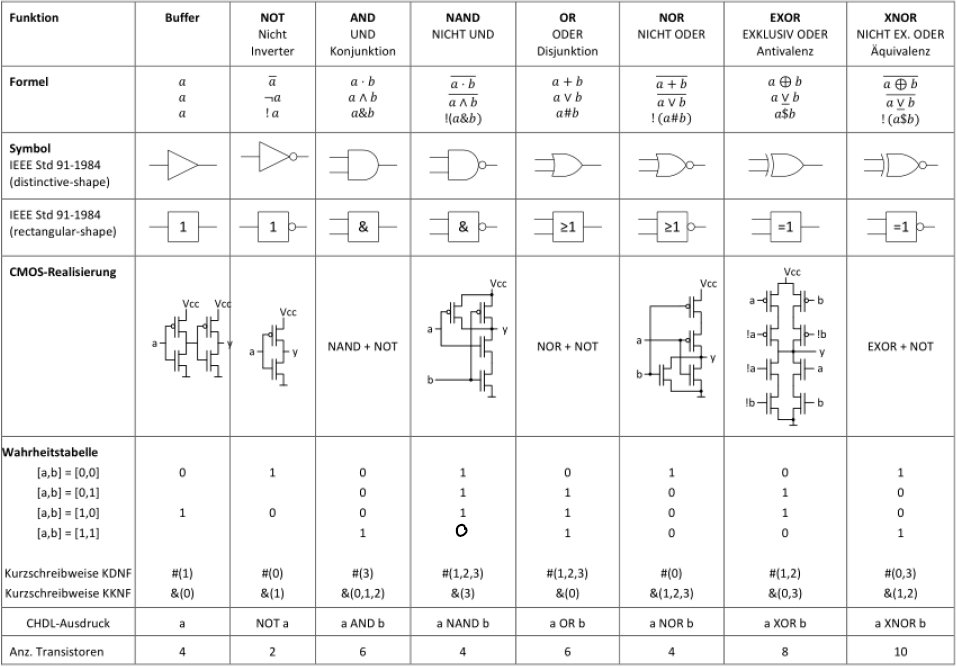
\includegraphics[width=19cm]{images/logische_operationen.png}
\subsection{Zahlenformate}
\begin{multicols}{2}
	\renewcommand{\arraystretch}{1.2}
	\begin{tabular}{|l|l|l|l|}
		\hline \textbf{Dezimal} & \textbf{Binär} & \textbf{Hexadezimal} & \textbf{Oktal}\\
		\hline 0 & 0000 & 0 & 0\\
		\hline 1 & 0001 & 1 & 1\\
		\hline 2 & 0010 & 2 & 2\\
		\hline 3 & 0011 & 3 & 3\\
		\hline 4 & 0100 & 4 & 4\\
		\hline 5 & 0101 & 5 & 5\\
		\hline 6 & 0110 & 6 & 6\\
		\hline 7 & 0111 & 7 & 7\\
		\hline 8 & 1000 & 8 & 0\\
		\hline 9 & 1001 & 9 & 0\\
		\hline 10 & 1010 & A & 0\\
		\hline 11 & 1011 & B & 0\\
		\hline 12 & 1100 & C & 0\\
		\hline 13 & 1101 & D & 0\\
		\hline 14 & 1110 & E & 0\\
		\hline 15 & 1111 & F & 0\\
		\hline
	\end{tabular}

\subsection{2er-Potenzen}
\begin{tabular}{|l|l|}
			\hline $2^0$ & $1$\\
			\hline $2^1$ & $2$\\
			\hline $2^2$ & $4$\\
			\hline $2^3$ & $8$\\
			\hline $2^4$ & $16$\\
			\hline $2^5$ & $32$\\
			\hline $2^6$ & $64$\\
			\hline $2^7$ & $128$\\
			\hline $2^8$ & $256$\\
			\hline $2^9$ & $512$\\
			\hline $2^{10}$ & $1024$\\
			\hline $2^{20}$ & $1 M$\\
			\hline $2^{30}$ & $1 G$\\
			\hline $2^{24}$ & $2^{20} +2^4 = 1M \cdot 16 = 16M$\\
			\hline
\end{tabular}
\end{multicols}
\clearpage
\pagebreak